\chapter*{Abstract}

One of the most amazing capabilities of human beings is to extract common spatial patterns from observations and use these patterns to make inferences - recognizing a car by summarizing the important components of cars, like rims, windows, trunks etc., and their spatial relationship while ignoring the specific design of different cars. 

\begin{figure}[h]
	\centering
	\captionsetup{justification=centering}
	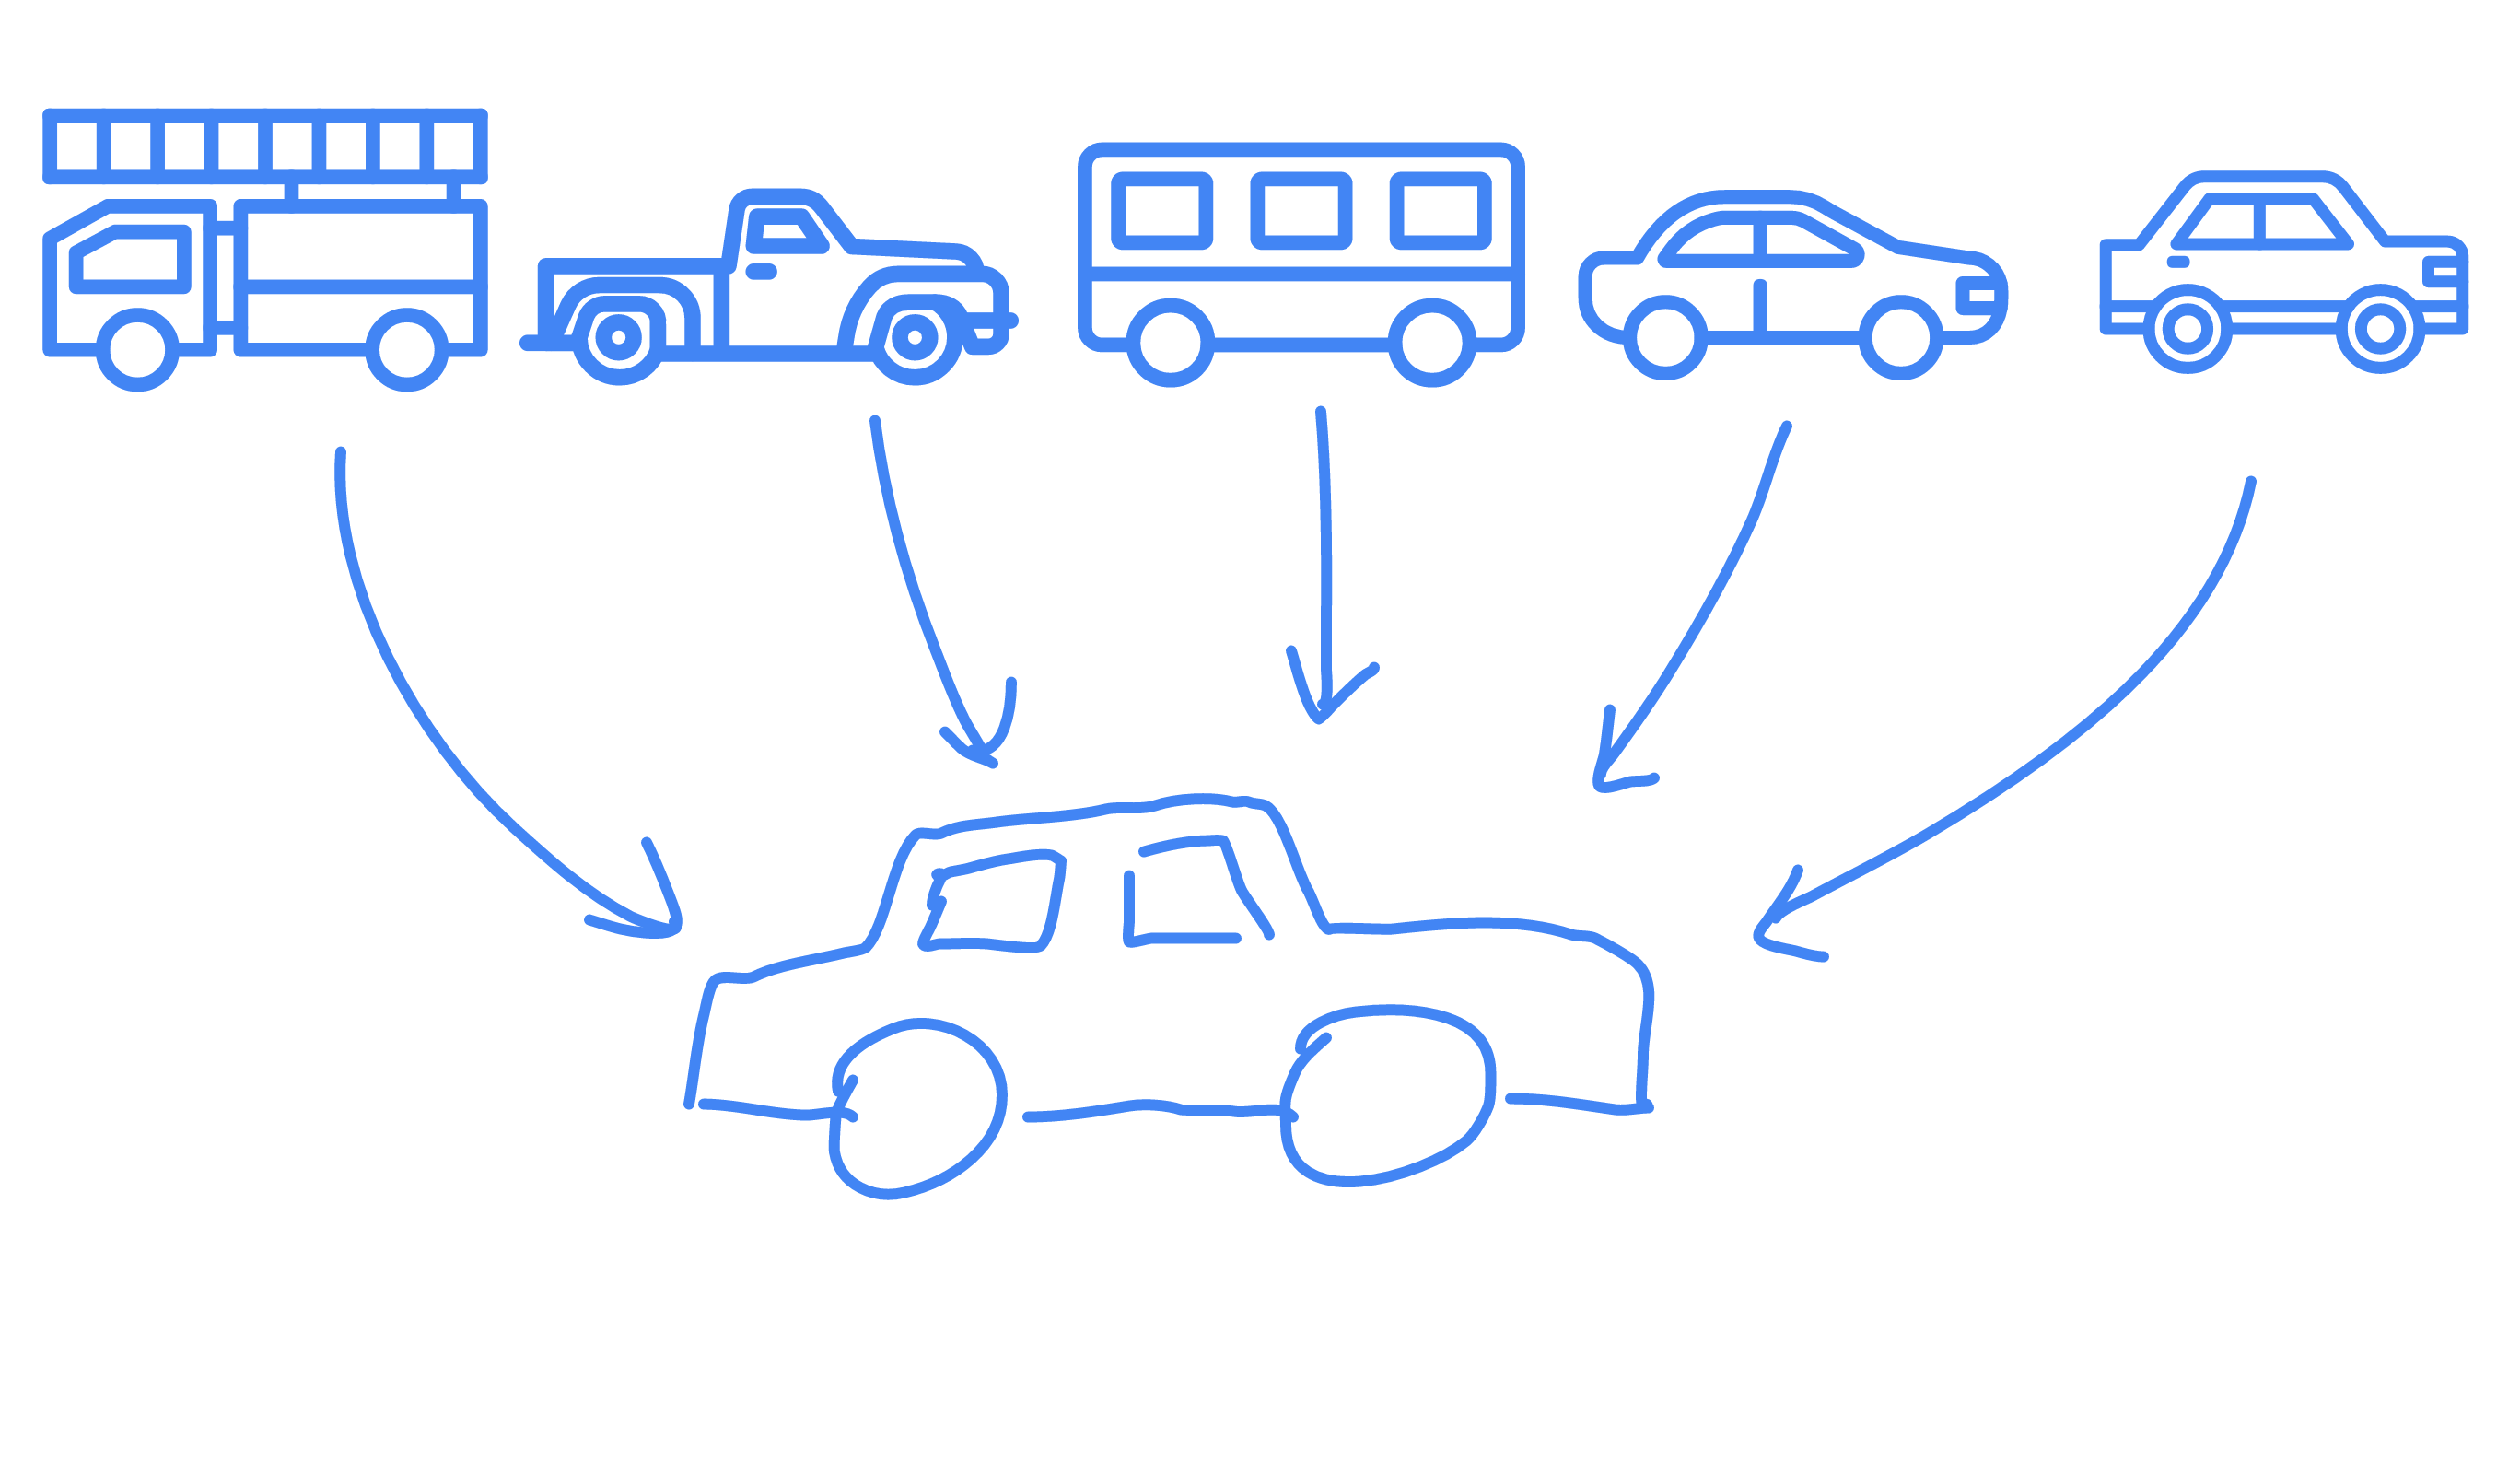
\includegraphics[width=0.6\textwidth]{figs/car_summary.png}
	\caption[Caption for LOF]{\emph{Different cars can be summarized as some simple components in a certain spatial relationship.\footnotemark}}
	\label{fig:car_summary}
\end{figure}
\footnotetext{The figure is drawn by a tool called Autodraw developed by Google using machine learning techniques.}

In our work, we turn a set of spatial representations into a set of attributed relational graphs (ARGs), which consist of nodes and edges with a vector representing their individual features. We then train a probabilistic parametric model that extract the common sub-graph of the ARGs set.\\

Our key contributions are 1) introducing a stochastic process to the graph matching step which utilizes a graduated assignment algorithm, 2) adding a null node network in each ARG to avoid matches among background nodes (i.e. nodes not in the pattern). We also apply the model to crystallography protein structure data to learn the common structure among proteins that share a certain function. To utilize the general algorithm to our protein data and model the structure data as ARG, we 3) introduce an additional term in our objective function representing the protein backbone, and 4) use a local substitution vector to model the similarity between two different amino acids based on their specific local environment.\\

Graph is a powerful representation and can be used to model a lot of things like neuron morphologies and social networks. Utilizing such algorithm can help machines to understand many of the patterns in real life, and human to mine pattern in large scale.

\chapter*{Acknowledgments}

This work was supported by the Jerome A. Schiff Fellowship, and advised by Prof. Pengyu Hong at Brandeis University.\\

Prof. Hong gave me a change in the summer of 2015, and asked me to implement some pre-existing algorithms in MATLAB. We then modified this algorithm to handle some issues that occurred with larger graphs. After we fixed the issues, we applied the modified algorithm to protein structure data which in this work. I thank Prof. Hong for his continuous support, inspiration, and guidance along this amazing journey.\\

I came to Brandeis University as a math major, but the magical intro lecture by Prof. Antonella DiLillo led me to the computer science major instead. The JBS program led by Prof. Timothy J. Hickey and Prof. Marie M. Meteer allowed me to build an Siri-like app and introduced me to this amazing AI world. Prof. Harry Mairson introduced the beauty of simplicity to me, while courses taught by Prof. Mitch Cherniack and Prof. Liuba Shrira helped me appreciate such simplicity in even the most powerful and complex systems. Such "deconstruction" mindset guided me through many obstacles along this research journey. There are many other mentors at Brandeis helped me appreciate what I do and inspired me to do great work in the future, so I also want to give a special shout out to this warm welcoming community.\\

Last but not least, I want to thank my family, friends, and Netflix for distracting me from research and being the scapegoats for my own procrastination.